\documentclass{article}

\usepackage[utf8]{inputenc}
\usepackage[top=1.5in,left=1in,right=1in,bottom=1.5in,headheight=1in]{geometry}
\usepackage{fancyhdr}
\usepackage{amsmath,amsthm,amsfonts}
\usepackage{setspace}
\usepackage{multicol}
\usepackage{tikz}

\onehalfspacing

% \theoremstyle{theorem}
\newtheorem*{thm}{Theorem}
\renewcommand\qedsymbol{}

%%% Heading -- No need to edit %%%
\pagestyle{fancy}
\rhead{
Stefan Eng \\ 
Dr. Katherine Stevenson \\ 
Math320 \\ 
9/16/13
}
%%%

\begin{document}
\pagenumbering{gobble}

%%% Make the title %%%
\begin{center}
\textsc{\Large Foundations of Higher Mathematics}\\[.3cm]
\textsc{\Large Journal 3}\\[1cm]
\end{center}
%%% End title %%%

%%% Start Journal Here Here %%%

\section*{One, Two, Three \ldots Infinity (Part 1)}

So I took your advice and read the first part of One, Two, Three, Infinity and it has been fascinating so far. If you have any more recommendations I would love to hear them. Gamow's slightly less formal approach to infinity way a great way to learn about some of the concepts. There were three examples that stood out in the first part of this book that really were quiet amazing. They all involved points and the infinite set $\aleph_1$. These examples were first recognized by Georg Cantor, who created the method for comparing two infinities and modern set theory. His creative method of showing that \textit{the number of all point on a plane is equal to the number of points on a line} really amazed me.

\subsection*{Example}
I refer to this as a theorem and proof but it is more informal. I tried to get the feel and method that Gamow was trying to convey in my own words.
\begin{thm}
The number of all points on a plane is equal to the number of points on a line
\end{thm}

\begin{multicols}{2}
  \begin{proof}
    Given a line, we can treat any point on the line as some number in $\mathbb{R}$ between zero and one. For a plane, each point on the plane can be represented as an pair of points in $\mathbb{R}$, between zero and one. We can map each point on line to the plane from the sphere by taking every odd decimal point for the y values, and every even decimal place for the x values, as seen in the picture to the right. To map the points on the plane to the line, we \textit{merge} the two decimal places by alternating which decimal we take from, and make the two points into one. 
\begin{align*}
&.1\ \ \ 3\ \ \ 5\ \ \ 7 \\
&\downarrow \nearrow \downarrow \nearrow \downarrow \nearrow \downarrow\\
&.2\ \ \ 4\ \ \ 6\ \ \ 8\\
&= .12345678
\end{align*}
Thus, since we have a one-to-one mapping of all points, the points on the plane have the same number of points as the line does.
  \end{proof}
  \begin{center}
    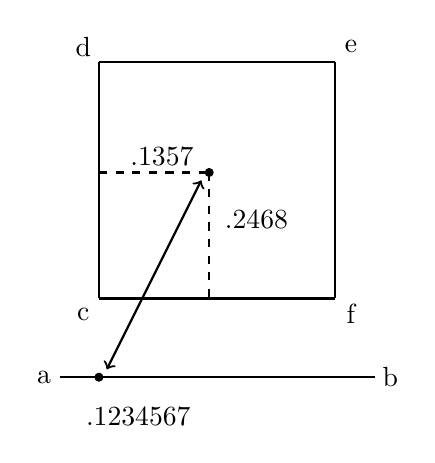
\begin{tikzpicture}
      %\draw[help lines] (0,0) grid (5,5);,
      % Square
      \node at (.8,1.8) {c};
      \draw[thick] (1,2) -- (1,5);
      \node at (.8,5.2) {d};
      \draw[thick] (1,5) -- (4,5);      
      \node at (4.2,5.2) {e};
      \draw[thick] (4,5) -- (4,2);     
      \node at (4.2,1.8) {f};
      \draw[thick] (4,2) -- (1,2);
      % Line
      \draw[thick] (.5,1) -- (4.5,1);      
      \node at (.3,1) {a};
      \node at (4.7,1) {b};
      \node at (1.5,.5) {.1234567};
      \draw[fill] (1,1) circle [radius=.05];
      % Inner square
      \draw[thick, dashed] (1,3.6) -- (2.4,3.6);
      \node at (1.8,3.8) {.1357};
      \draw[fill] (2.4,3.6) circle [radius=.05];
      \draw[thick, dashed] (2.4,3.6) -- (2.4,2);
      \node at (3,3) {.2468};
      % Line connecting the two
      \draw[thick, <->] (1.1,1.1) -- (2.3,3.5);
    \end{tikzpicture}
  \end{center}
\end{multicols}




\end{document}

%%% End assignment %%%